\documentclass{article}\usepackage[]{graphicx}\usepackage[]{xcolor}
% maxwidth is the original width if it is less than linewidth
% otherwise use linewidth (to make sure the graphics do not exceed the margin)
\makeatletter
\def\maxwidth{ %
  \ifdim\Gin@nat@width>\linewidth
    \linewidth
  \else
    \Gin@nat@width
  \fi
}
\makeatother

\definecolor{fgcolor}{rgb}{0.345, 0.345, 0.345}
\newcommand{\hlnum}[1]{\textcolor[rgb]{0.686,0.059,0.569}{#1}}%
\newcommand{\hlstr}[1]{\textcolor[rgb]{0.192,0.494,0.8}{#1}}%
\newcommand{\hlcom}[1]{\textcolor[rgb]{0.678,0.584,0.686}{\textit{#1}}}%
\newcommand{\hlopt}[1]{\textcolor[rgb]{0,0,0}{#1}}%
\newcommand{\hlstd}[1]{\textcolor[rgb]{0.345,0.345,0.345}{#1}}%
\newcommand{\hlkwa}[1]{\textcolor[rgb]{0.161,0.373,0.58}{\textbf{#1}}}%
\newcommand{\hlkwb}[1]{\textcolor[rgb]{0.69,0.353,0.396}{#1}}%
\newcommand{\hlkwc}[1]{\textcolor[rgb]{0.333,0.667,0.333}{#1}}%
\newcommand{\hlkwd}[1]{\textcolor[rgb]{0.737,0.353,0.396}{\textbf{#1}}}%
\let\hlipl\hlkwb

\usepackage{framed}
\makeatletter
\newenvironment{kframe}{%
 \def\at@end@of@kframe{}%
 \ifinner\ifhmode%
  \def\at@end@of@kframe{\end{minipage}}%
  \begin{minipage}{\columnwidth}%
 \fi\fi%
 \def\FrameCommand##1{\hskip\@totalleftmargin \hskip-\fboxsep
 \colorbox{shadecolor}{##1}\hskip-\fboxsep
     % There is no \\@totalrightmargin, so:
     \hskip-\linewidth \hskip-\@totalleftmargin \hskip\columnwidth}%
 \MakeFramed {\advance\hsize-\width
   \@totalleftmargin\z@ \linewidth\hsize
   \@setminipage}}%
 {\par\unskip\endMakeFramed%
 \at@end@of@kframe}
\makeatother

\definecolor{shadecolor}{rgb}{.97, .97, .97}
\definecolor{messagecolor}{rgb}{0, 0, 0}
\definecolor{warningcolor}{rgb}{1, 0, 1}
\definecolor{errorcolor}{rgb}{1, 0, 0}
\newenvironment{knitrout}{}{} % an empty environment to be redefined in TeX

\usepackage{alltt}
\usepackage{amsmath}
\usepackage{enumerate}
\usepackage{listings}
\usepackage{natbib}[numbers, sort&compress]
\setcitestyle{numbers,open={[},close={]}}
\usepackage{url}

\newcommand{\rcode}[1]{\lstinline[language=R,basicstyle=\normalsize\ttfamily]!#1!}
\setcounter{section}{1}

%\VignetteEngine{knitr::knitr}
%\VignetteIndexEntry{Examples}

\title{Fitting a zeta distribution to a {P} survey---number of groups data}
\IfFileExists{upquote.sty}{\usepackage{upquote}}{}
\begin{document}



We have, as noted throughout this paper, tried to make the statistical methodology as accessible as possible by implementing it in an R package. In this section we will demonstrate the use of the package with data from various surveys.

\subsection{Fitting a zeta distribution}
We start with the data from \citet{roux2001} who conducted a footwear survey, where shoes from 776 individuals were examined for glass. This data set is built into the package and can be accessed from the \rcode{Psurveys} object. That is, we can type:
\begin{knitrout}
\definecolor{shadecolor}{rgb}{0.969, 0.969, 0.969}\color{fgcolor}\begin{kframe}
\begin{alltt}
\hlstd{> }\hlkwd{data}\hlstd{(}\hlstr{"Psurveys"}\hlstd{)}
\hlstd{> }\hlstd{roux} \hlkwb{=} \hlstd{Psurveys}\hlopt{$}\hlstd{roux}
\end{alltt}
\end{kframe}
\end{knitrout}
The package includes a special printing function that summarises the data for reading rather than displaying it in the way it is stored. R prints the values of objects (or variables) simply by typing their name. For example
\begin{knitrout}
\definecolor{shadecolor}{rgb}{0.969, 0.969, 0.969}\color{fgcolor}\begin{kframe}
\begin{alltt}
\hlstd{> }\hlstd{roux}
\end{alltt}
\begin{verbatim}
Number of Groups

  n    rn
---  ----
  0   754
  1     9
  2     8
  3     4
  4     1
Roux C, Kirk R, Benson S, Van Haren T, Petterd C (2001).
"Glass particles in footwear of members of the public in
south-eastern Australia-a survey." _Forensic Science
International_, *116*(2), 149-156.
doi:10.1016/S0379-0738(00)00355-8
<https://doi.org/10.1016/S0379-0738%2800%2900355-8>.
\end{verbatim}
\end{kframe}
\end{knitrout}
It is very simple to fit a zeta distribution to this data set. We do this using the \rcode{fitDist} function.
\begin{knitrout}
\definecolor{shadecolor}{rgb}{0.969, 0.969, 0.969}\color{fgcolor}\begin{kframe}
\begin{alltt}
\hlstd{> }\hlstd{fit} \hlkwb{=} \hlkwd{fitDist}\hlstd{(roux)}
\end{alltt}
\end{kframe}
\end{knitrout}
There is nothing special about the variable name \rcode{fit}. It could be anything, for example \rcode{x}, or \rcode{blah}. However we choose the variable name \rcode{fit} because it is easy to remember that it is a \emph{fitted} object. The package includes specialised functions for both printing and plotting the fitted object. The \rcode{print} method displays an estimate of the shape parameter $\alpha$, an estimate of the standard deviation---the standard error---of the estimate of $\alpha$ ($\widehat{\mathrm{sd}}(\hat{\alpha})=\mathrm{se}(\hat{\alpha})$). \textbf{Note:} it is important to understand that the value of the shape parameter that is displayed, and the value that is stored in the fitted object differ by 1. That is, $\alpha$ is shown, and $s = \alpha - 1$ is stored. This difference only has consequences if the fitted value is being used in conjunction with other functions.

\subsubsection{Using the fitted distribution to estimate $P$ terms}
The \rcode{print} method also displays the first 10 fitted probabilities from the model by default.
\begin{knitrout}
\definecolor{shadecolor}{rgb}{0.969, 0.969, 0.969}\color{fgcolor}\begin{kframe}
\begin{alltt}
\hlstd{> }\hlstd{fit}
\end{alltt}
\begin{verbatim}
The estimated shape parameter is 4.9544 
The standard error of shape parameter is 0.2366 
------
NOTE: The shape parameter is reported so that it is consistent
with Coulson et al. However, the value returned is actually s'
= shape - 1 to be consistent with the VGAM parameterisation,
which is used for computation. This has flow on effects, for
example in confInt. This will be changed at some point.
------

The first  10 fitted values are:
          P0           P1           P2           P3           P4 
9.631547e-01 3.106447e-02 4.167082e-03 1.001917e-03 3.316637e-04 
          P5           P6           P7           P8           P9 
1.344002e-04 6.262053e-05 3.231467e-05 1.802885e-05 1.069709e-05 
\end{verbatim}
\end{kframe}
\end{knitrout}
This information is probably sufficient for most casework. However, the package has a function, \rcode{probfun}, that returns a bespoke function that can calculate any probability term. This function is applied a fitted object. For example
\begin{knitrout}
\definecolor{shadecolor}{rgb}{0.969, 0.969, 0.969}\color{fgcolor}\begin{kframe}
\begin{alltt}
\hlstd{> }\hlstd{P} \hlkwb{=} \hlkwd{probfun}\hlstd{(fit)}
\end{alltt}
\end{kframe}
\end{knitrout}
Again, \rcode{P} is just a variable name and we could have used anything. We have chosen \rcode{P} because this probability function returns $P$ terms. To use it, we type only need to provide the value of $k$, and the function will return $P_k$. For example
\begin{knitrout}
\definecolor{shadecolor}{rgb}{0.969, 0.969, 0.969}\color{fgcolor}\begin{kframe}
\begin{alltt}
\hlstd{> }\hlkwd{P}\hlstd{(}\hlnum{5}\hlstd{)}
\end{alltt}
\begin{verbatim}
          P5 
0.0001344002 
\end{verbatim}
\end{kframe}
\end{knitrout}

\subsection{Fitting a zero-inflated zeta distribution}
We can also easily fit a zero-inflated zeta model using the \rcode{fitZIDist} function\footnote{Functions with mixed case names are often annoying. For that reason, the package also allows \rcode{fitZIdist} and \rcode{fitzidist}.}. As before, we can choose a variable name to store the results in.
\begin{knitrout}
\definecolor{shadecolor}{rgb}{0.969, 0.969, 0.969}\color{fgcolor}\begin{kframe}
\begin{alltt}
\hlstd{> }\hlstd{fit.zi} \hlkwb{=} \hlkwd{fitZIDist}\hlstd{(roux)}
\hlstd{> }\hlstd{fit.zi}
\end{alltt}
\begin{verbatim}
The estimated mixing parameter, pi, is 0.8465 
The estimated shape parameter is 2.8846 
------
NOTE: The shape parameter is reported so that it is consistent
with Coulson et al. However, the value returned is actually s'
= shape - 1 to be consistent with the VGAM parameterisation,
which is used for computation. This has flow on effects, for
example in confInt. This will be changed at some point.
------

The first  10 fitted values are:
          P0           P1           P2           P3           P4 
0.9716490911 0.0169404164 0.0052597614 0.0022938450 0.0012050764 
          P5           P6           P7           P8           P9 
0.0007122067 0.0004565511 0.0003106019 0.0002211302 0.0001631754 
\end{verbatim}
\end{kframe}
\end{knitrout}
In the example above we fit a zero-inflated model to Roux et al.'s data, and print out the resulting fit. We get, as with the zeta model, estimates of the parameters and a default set of fitted values. The output is interesting in that we can see (from the value of $\hat{\pi}$) that the \emph{zero} part of the zero-inflated model is picking up about 85\% of the zeros. It is interesting to compare the estimates from the raw frequencies, the zeta model, and those of the ZIZ model. The estimates are shown in Table \ref{tab:ex1}.
% latex table generated in R 4.3.2 by xtable 1.8-4 package
% Tue Jan  9 15:50:44 2024
\begin{table}[ht]
\centering
\begin{tabular}{cccc}
  \hline
$k$ & $P_k^{raw}$ & $P_k^{zeta}$ & $P_k^{ZIZ}$ \\ 
  \hline
0 & 0.9716 & 0.9632 & 0.9716 \\ 
  1 & 0.0116 & 0.0311 & 0.0169 \\ 
  2 & 0.0103 & 0.0042 & 0.0053 \\ 
  3 & 0.0052 & 0.0010 & 0.0023 \\ 
  4 & 0.0013 & 0.0003 & 0.0012 \\ 
  5 & 0.0000 & 0.0001 & 0.0007 \\ 
   \hline
\end{tabular}
\caption{Estimated probability that $k$ groups of glass would be found in shoes of a random member of the population based on the data of \citep{roux2001}, the raw frequencies, and those produced from the zeta and ZIZ models respectively.} 
\label{tab:ex1}
\end{table}

We can see from Table \ref{tab:ex1} that we now have a non-zero estimate for $P_5$,
but this comes at a small cost, namely smaller probabilities for the preceding terms $P_0$--$P_4$. This is not necessarily a negative. The survey data is dominated by zeros. However, we think it likely that the raw sample estimates (for $P_0$--$P_4$) are over-estimates. The model reduces the estimated value, which is in line with our thinking. Interestingly, the effect of including the zero-inflation factor is to increase nearly all of the probabilities, with the exception of $P_1$. A natural question to ask is ``Which model is correct?'' The answer, unhelpfully, is ``Neither.'' This is because these are simply models. They can still help us without us having to believe that they are true.

\subsection{Confidence intervals for the parameter estimates}
The \texttt{fitPS} package provides a \rcode{confint} method for the fitted value. The method returns both a Wald confidence interval and profile likelihood interval. The two intervals are returned as elements of a \rcode{list} named \rcode{wald} and \rcode{prof} respectively.
\begin{knitrout}
\definecolor{shadecolor}{rgb}{0.969, 0.969, 0.969}\color{fgcolor}\begin{kframe}
\begin{alltt}
\hlstd{> }\hlstd{ci} \hlkwb{=} \hlkwd{confint}\hlstd{(fit)}
\hlstd{> }\hlstd{ci}\hlopt{$}\hlstd{wald}
\end{alltt}
\begin{verbatim}
    2.5%    97.5% 
3.490761 4.418099 
\end{verbatim}
\begin{alltt}
\hlstd{> }\hlstd{ci}\hlopt{$}\hlstd{prof}
\end{alltt}
\begin{verbatim}
    2.5%    97.5% 
3.520495 4.451277 
\end{verbatim}
\end{kframe}
\end{knitrout}
Readers may notice neither of these intervals contain the estimated value shown in the previous output. However, this simply because they are confidence intervals on $s^\prime$ and not $s$. This can be remedied by adding one to each interval:
\begin{knitrout}
\definecolor{shadecolor}{rgb}{0.969, 0.969, 0.969}\color{fgcolor}\begin{kframe}
\begin{alltt}
\hlstd{> }\hlstd{ci}\hlopt{$}\hlstd{wald} \hlopt{+} \hlnum{1}
\end{alltt}
\begin{verbatim}
    2.5%    97.5% 
4.490761 5.418099 
\end{verbatim}
\begin{alltt}
\hlstd{> }\hlstd{ci}\hlopt{$}\hlstd{prof} \hlopt{+} \hlnum{1}
\end{alltt}
\begin{verbatim}
    2.5%    97.5% 
4.520495 5.451277 
\end{verbatim}
\end{kframe}
\end{knitrout}
The reason for not \emph{correcting} these intervals is that the method mostly exists to feed into other parts of the package, especially the \rcode{plot} method.

\subsubsection{Bootstrapped and profile likelihood confidence regions for the zero-inflated zeta}
The package includes the facility to compute both bootstrapped and profile likelihood confidence regions for the parameters of the zero-inflated zeta distribtion. It does, also, in fact compute bootstrapped confidence intervals for the zeta distribution, but we do not do demonstrate this functionality here. The \rcode{confint} function returns a confidence region if the fitted object contains information from a zero-inflated zeta fit. As an example, we will first compute profile likelihood confidence regions for the \citet{roux2001} data. To do this we use the fitted object we previously created, \rcode{fit.zi}, and, although not required, we supply a set of two levels so that we can compute both an 80\% and a 95\% confidence region. \rcode{confit} returns a list of confidence regions---one for each level---each of which are simply a set of $x$ and $y$ coordinates corresponding to the appropriate contour line. We can use this information for plotting. The code to produce Figure \ref{fig:confregion} is given below.
\begin{knitrout}
\definecolor{shadecolor}{rgb}{0.969, 0.969, 0.969}\color{fgcolor}\begin{kframe}
\begin{alltt}
\hlstd{> }\hlstd{cr} \hlkwb{=} \hlkwd{confint}\hlstd{(fit.zi,} \hlkwc{level} \hlstd{=} \hlkwd{c}\hlstd{(}\hlnum{0.80}\hlstd{,} \hlnum{0.95}\hlstd{))}
\hlstd{> }\hlkwd{plot}\hlstd{(cr[[}\hlstr{"0.95"}\hlstd{]],} \hlkwc{type} \hlstd{=} \hlstr{"l"}\hlstd{)}
\hlstd{> }\hlkwd{polygon}\hlstd{(cr[[}\hlstr{"0.8"}\hlstd{]],} \hlkwc{border} \hlstd{=} \hlstr{"red"}\hlstd{)}
\hlstd{> }\hlkwd{legend}\hlstd{(}\hlstr{"topright"}\hlstd{,} \hlkwc{lty} \hlstd{=} \hlnum{1}\hlstd{,} \hlkwc{lwd} \hlstd{=} \hlnum{2}\hlstd{,} \hlkwc{col} \hlstd{=} \hlkwd{c}\hlstd{(}\hlstr{"red"}\hlstd{,} \hlstr{"black"}\hlstd{),}
\hlstd{+ }       \hlkwc{legend} \hlstd{=} \hlkwd{c}\hlstd{(}\hlstr{"80%"}\hlstd{,} \hlstr{"95%"}\hlstd{),} \hlkwc{bty} \hlstd{=} \hlstr{"n"}\hlstd{)}
\end{alltt}
\end{kframe}
\end{knitrout}

\begin{figure}[ht]
\centering
  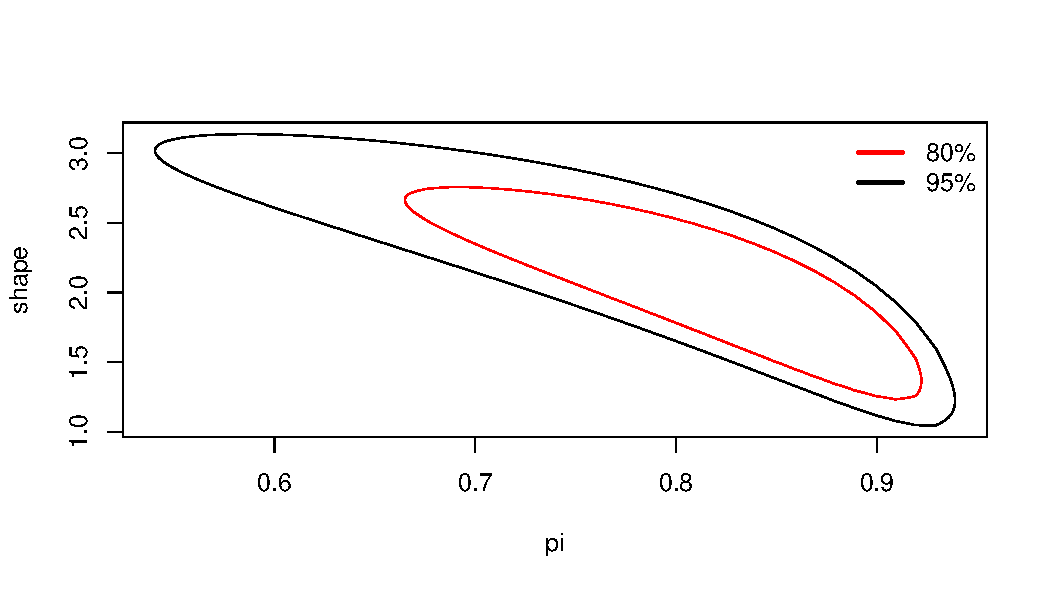
\includegraphics[width=0.95\textwidth,keepaspectratio]{confregion}
  \caption{80\% and 95\% confidence regions for the parameters of a zero-inflated zeta distribution fitted to the \citet{roux2001} data.}
  \label{fig:confregion}
\end{figure}
A bootstrapped confidence region can be computed using the \rcode{bootCI} function. The \rcode{bootCI} function includes the facility to plot the resulting confidence
region(s) as and hide or display the function's progress. The latter is important because this procedure is numerically intensive, and even with utilising parallel processing, can be quite slow. The code below produces Figure \ref{fig:bootconfregion}
\begin{knitrout}
\definecolor{shadecolor}{rgb}{0.969, 0.969, 0.969}\color{fgcolor}\begin{kframe}
\begin{alltt}
\hlstd{> }\hlstd{bcr} \hlkwb{=} \hlkwd{bootCI}\hlstd{(roux,} \hlkwc{model} \hlstd{=} \hlstr{"ziz"}\hlstd{,} \hlkwc{plot} \hlstd{=} \hlnum{TRUE}\hlstd{,} \hlkwc{silent} \hlstd{=} \hlnum{TRUE}\hlstd{)}
\end{alltt}
\end{kframe}
\end{knitrout}

\begin{figure}[ht]
\centering
  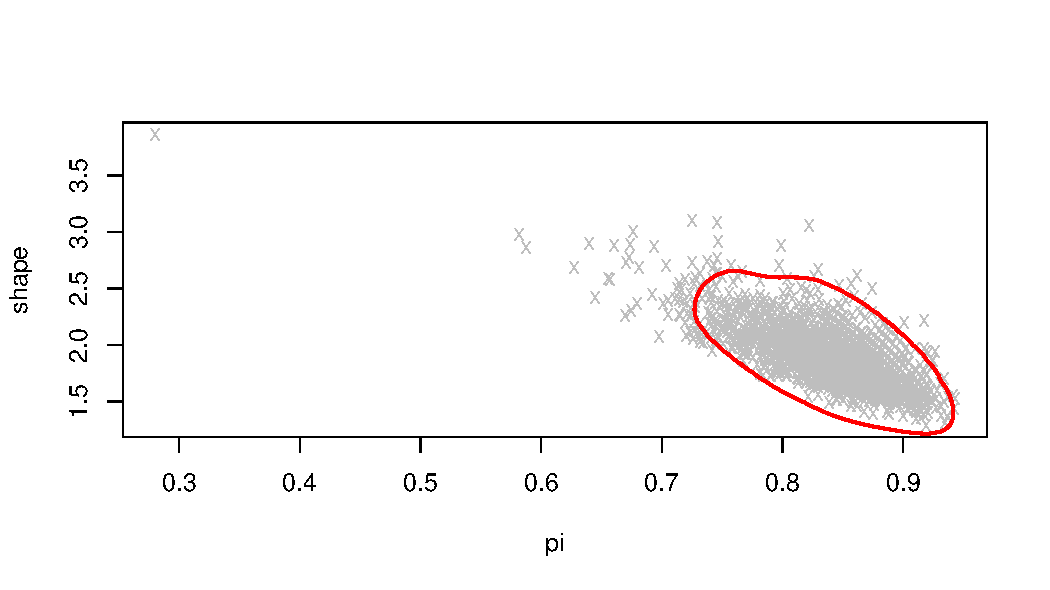
\includegraphics[width=0.95\textwidth,keepaspectratio]{bootconfregion}
  \caption{A 95\% bootstrapped confidence region for the parameters of a zero-inflated zeta distribution fitted to the \citet{roux2001} data.}
  \label{fig:bootconfregion}
\end{figure}

\subsection{Comparing two surveys}
We can use the methodology that has been demonstrated so far to compare surveys. One reason for comparing surveys is to explore the hypothesis that there is no difference in the underlying ``true\footnote{Readers may be aware that one of the authors is fundementally Bayesian at heart, and the so the concept of the true value of a population parameter is antithetical to the school of thought. We, however, proceed on the basis that the Frequenist school of thought is not incorrect, but just differs in interpretation.}'' value of $\alpha$. If there is insufficient evidence to reject this hypothesis, then one may feel justified in combining data from two surveys. In the first instance we will take an ad-hoc approach, and then treat this problem more formally. In our ad-hoc approach we will compare confidence intervals for two-surveys. If these confidence intervals overlap, then we might conclude that there is insufficient evidence in the data to suggest that the estimates of $\alpha$ are different. We will illustrate this with the surveys conducted by \citet{lau1997} and \citet{jackson2013}. \citet{lau1997} surveyed the clothing of 213 Canadian high school students and observed two sets of clothing with one fragment on each. Similarly, \citet{jackson2013} surveyed 232 ``randomly'' selected members of the population of New South Wales in Australia. We place ``randomly'' in quotes because this was not a true random sample, but rather a convenience sample. That being said, it is unlikely that using a truly random mechanism would have significantly changed the results. \citet{jackson2013} found a single fragment of glass on each of six people. The data from each of these two surveys is summarised in Table \ref{tab:lau_and_jackson}.
% latex table generated in R 4.3.2 by xtable 1.8-4 package
% Tue Jan  9 15:50:45 2024
\begin{table}[ht]
\centering
\begin{tabular}{r|r|r}
  \multicolumn{1}{c}{} & \multicolumn{2}{c}{$r_n$} \\  $n$ & Lau et al. & Jackson et al.  \\ \hline
0 & 211 & 224 \\ 
  1 & 2 & 6 \\ 
  \end{tabular}
\caption{Survey results from \citet{lau1997} and \citet{jackson2013}.} 
\label{tab:lau_and_jackson}
\end{table}

Visual inspection of these surveys would suggest that they are fairly similar. We can fit a zeta distribution to each survey, and then compute a confidence interval for each survey. Again, these data sets are included in the \texttt{fitPS} package.
\begin{knitrout}
\definecolor{shadecolor}{rgb}{0.969, 0.969, 0.969}\color{fgcolor}\begin{kframe}
\begin{alltt}
\hlstd{> }\hlstd{lau} \hlkwb{=} \hlstd{Psurveys}\hlopt{$}\hlstd{lau}
\hlstd{> }\hlstd{jackson} \hlkwb{=} \hlstd{Psurveys}\hlopt{$}\hlstd{jackson}
\hlstd{> }\hlstd{fit.lau} \hlkwb{=} \hlkwd{fitDist}\hlstd{(lau)}
\hlstd{> }\hlstd{fit.jackson} \hlkwb{=} \hlkwd{fitDist}\hlstd{(jackson)}
\hlstd{> }\hlkwd{confint}\hlstd{(fit.lau)}\hlopt{$}\hlstd{wald}
\end{alltt}
\begin{verbatim}
    2.5%    97.5% 
3.948422 7.823417 
\end{verbatim}
\begin{alltt}
\hlstd{> }\hlkwd{confint}\hlstd{(fit.jackson)}\hlopt{$}\hlstd{wald}
\end{alltt}
\begin{verbatim}
    2.5%    97.5% 
3.443639 5.623473 
\end{verbatim}
\end{kframe}
\end{knitrout}
We can see from the output that there is substantial overlap between these two (Wald) confidence intervals. The results using profile likelihood intervals lead to the same conclusion but are not shown. We can test this more formally. Specifically, we wish to test the (null) hypothesis that
\[
H_0:\alpha_{1} = \alpha_{2}\mbox{ or equivalently }H_0:\alpha_{1} - \alpha_{2} = 0,
\]
where $\alpha_1$ is the true value of $\alpha$ for the the Lau et al. data, and $\alpha_2$ is the true value of $\alpha$ for the the Jackson et al. data. We choose a two-tailed alternative, meaning we are not concerned about the sign of any difference, but simply the magnitude of the difference. That is,
\[
H_1:\alpha_{1} \neq \alpha_{2}\mbox{ or equivalently }H_1:\alpha_{1} - \alpha_{2} \neq 0.
\]
We test this hypothesis by constructing a test statistic, then computing a \emph{P}-value under the assumption that the null hypothesis is true. We are interested in the difference between the two population values of $\alpha$. We estimate this by computing the difference in the sample estimates. That is, our estimate of $\alpha_{1}-\alpha_{2}$, is given by $\hat{\alpha}_{1}-\hat{\alpha}_{2}$, where $\hat{\alpha}_{1}$ and $\hat{\alpha}_{2}$ are the maximum likelihood estimates based on the survey data. We scale this difference by the estimated standard deviation in the difference, that is, by the standard error of the difference, $se(\hat{\alpha}_{1}-\hat{\alpha}_{2})$. We estimate this---to keep the statistical theory to a minimum---as the sum of the square root of the two estimated variances, i.e.
\[
se(\hat{\alpha}_{1}-\hat{\alpha}_{2}) = \sqrt{\hat{V}(\hat{\alpha}_1)+\hat{V}(\hat{\alpha}_2)}.
\]
Our test statistic is then
\[
Z_0 = \frac{\hat{\alpha}_{1}-\hat{\alpha}_{2}}{se(\hat{\alpha}_{1}-\hat{\alpha}_{2})}.
\]
It can be shown that this test statistic follows an approximate normal distribution under the null hypothesis. That means we can compute our \emph{P}-value by evaluating
\begin{align*}
P&=\Pr(Z > |Z_0|) \\
&=2(1 - \Pr(Z < |Z_0|)).
\end{align*}
All this theory has been put in a function called \rcode{compareSurveys}
\begin{knitrout}
\definecolor{shadecolor}{rgb}{0.969, 0.969, 0.969}\color{fgcolor}\begin{kframe}
\begin{alltt}
\hlstd{> }\hlkwd{compareSurveys}\hlstd{(lau, jackson)}
\end{alltt}
\begin{verbatim}

	Two-sided Wald test

data:  lau and jackson
z = 1.1923, p-value = 0.2331
alternative hypothesis: true difference in shape parameters is not equal to 0
sample estimates:
    Shape of lau Shape of jackson 
        5.885919         4.533556 
\end{verbatim}
\end{kframe}
\end{knitrout}
We can see that the \emph{P}-value is 0.23 (2 d.p.). This is significantly larger than either 0.05, or 0.01. Based on this we would conclude that there is insufficient evidence to reject the null hypothesis of a common value of $\alpha$, and therefore it may be sensible to combine data from these two surveys. We could have also used the theory of likelihood ratio tests \citep{wiki:lrt} to test this hypothesis, but that is beyond the scope of this article. We note, however, that the \rcode{fitPS} package contains a function called \rcode{compareSurveysLRT} which can compare two \emph{or more} surveys simultaneously using a likelihood ratio test.
\bibliographystyle{unsrtnat}
\bibliography{references}
\end{document}
